
    \chapter*{5 Effizienz}
    \addcontentsline{toc}{chapter}{5 Effizienz}

    \begin{itemize}
        \item eine der zentralen Fragen bei Algorithmen
        \item Laufzeitmessung (\glqq wall clock time\grqq ): für den Endnutzer relevant
        \item Komplexität (auf abstrakt algorithmischer Ebene): für Programmierer \& Theoretiker
    \end{itemize}

    \section*{5.1 Laufzeit}
    \addcontentsline{toc}{section}{5.1 Laufzeit}
    \glqq der Algorithmus kommt $\underline{\text{rechtzeitig}}$ zum Ergebnis\grqq
    \begin{itemize}
        \item bei Steuerprogrammen (Maschinen, Fahrzeuge, Flugzeuge):
        \begin{itemize}
            \item mind. $< 1/1000$s Antwortzeit muss garantiert werden (nicht im Mittel, sondern immer) \glqq Echtzeit-Anforderung\grqq
            \item Video: 1/25s pro Bild für Dekompression
            \item Interaktion: nach 1/2 s muss etwas passieren, sonst klickt der Benutzer nochmals, zumindest Fortschrittsbalken
            \item Wettervorhersage: sollte fertig sein, $\underline{\text{bevor}}$ das reale Wetter passiert
        \end{itemize}
        \item Messung z.B. mit timeit-Modul (Python) Google benchmark (C/C++)
        \item wie erreicht man eine schnelle Laufzeit (außer: besseren Alg. wählen)
        \begin{itemize}
            \item in Python (langsame Sprache): in schnellere Sprachen auslagern (C, C++, Fortran)
            \begin{itemize}
                \item C-API (viele eingebaute Python-Module)
                \item Cython: schreibe (mit Python-Syntax $\Rightarrow$ wird automatisch kompiliert und eingebunden)
                \item pybind11 (Vorgänger: boost.python): Glue code generieren C/C++ (Glue code für Kommunikation zwischen Programmiersprachen notwendig)
            \end{itemize}
        \end{itemize}
        \item in kompilierten Sprachen (C, C++, Fortran) oder Sprachen mit Just-in-time Compiler (Java) kann man durch gute Code-Struktur eine Beschleunigung von 2x bis 10x erreichen.
        \begin{itemize}
            \item moderne Sprachen haben \glqq Optimierer\grqq , der den Code automatisch besser strukturiert
            \item $\underline{\text{Beispiele:}}$ \glqq common subexpression elimination\grqq : Doppelberechnungen vermeiden \\
            \begin{enumerate}
                \setcounter{enumi}{-1}
                \item $\underbrace{ x_1= -\frac{p}{2} + \sqrt{\frac{p^2}{4} - q}\hspace*{2mm}x_2= -\frac{p}{2} - \sqrt{\frac{p^2}{4} -q}}_{\text{nicht doppelt berechnen}}$
                \item $d = \sqrt{\frac{p^2}{4} - q}$,\hspace*{2mm} $x_1 = -\frac{p}{2} + d $,\hspace*{2mm} $x_2 =- \frac{p}{2} - d$
                \item $p2 = -\frac{p}{2}$, \hspace*{2mm}$d= \sqrt{p2**2-q}$,\hspace*{2mm} $x_1 = p2 + d$, \hspace*{2mm}$x_2 = p2 - d$
            \end{enumerate}
            \vspace*{2mm}
            \item \glqq loop invariant elimination\grqq : Ausdrücke, die in jeder Iteration dasselbe Ergebnis haben, aus der Schleife ziehen: Bsp.: Umrechnung von 2D Bildkoordinaten in 1D Speicherindizes
        \end{itemize}
        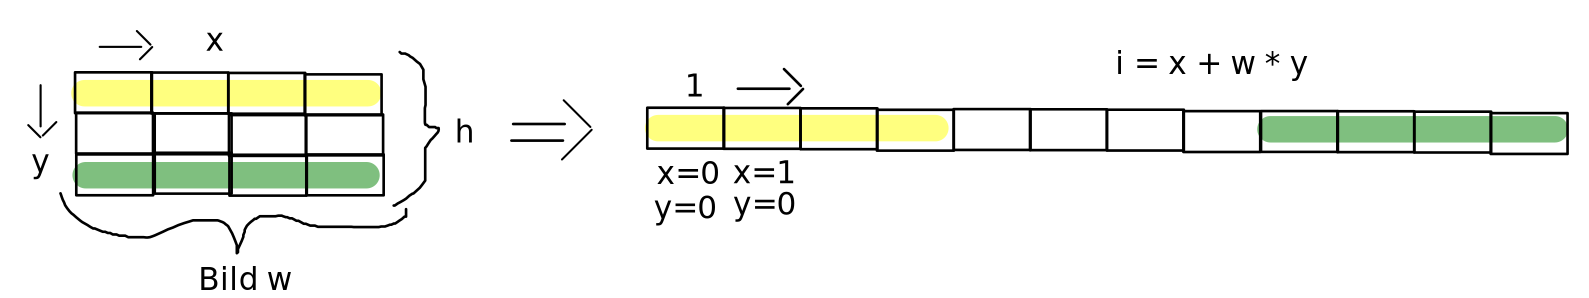
\includegraphics[width=15cm,height=8cm,keepaspectratio]{./Pictures/2D1D.png}
        \begin{minted}{python}
        for y in range(h):
            for x in range(w):
                data[x+w*y] = 0 #Initialisierung
        #Optimierung:
        for y in range(h):
            wy = w * y
            for x in range(w):
                data[x+wy]=0
        \end{minted}
        Faustregel: \glqq Vereinfachung der inneren Schleife\grqq  (wird am meisten ausgeführt)\\
        Ausnutzen der Hardware:
        \begin{itemize}
            \item Prozessor Cache: Kommunikation zwischen CPU und RAM ist langsam
            \begin{itemize}[label={$\Rightarrow$}]
                \item naiver Code: CPU wartet häufig auf RAM-Zugriff
                \item Cache Zugriffe sind schnell  $\Rightarrow$ sorge dafür, dass benötigte Daten bereits im Cache sind $\widehat{=}$ Daten, die im Speicher in der Nähe der bereits bearbeiteten Daten liegen \glqq cache locality\grqq
                \item strukturiere Schleifen so, dass in der inneren Schleife auf aufeinanderfolgende Daten zugegriffen wird
            \end{itemize}
            \item Prozessor Pipeline: jeder Befehl besteht aus Phasen, z.B.
        \end{itemize}
    \end{itemize}
    \begin{figure}[htbp]
        \begin{minipage}[t]{7cm}
            \vspace*{-2cm}
            \begin{enumerate}
                \item Dekodieren des Befehls
                \item Beschaffen der Inputdaten
                \item Ausführen des Befehls
                \item Abspeichern des Ergebnisses
            \end{enumerate}
        \end{minipage}
        \begin{minipage}{6cm}
        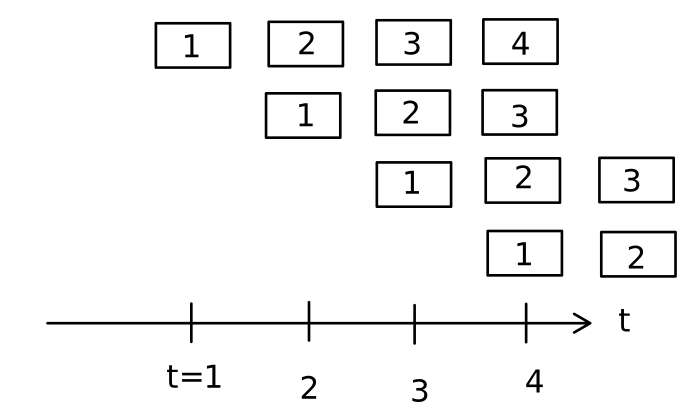
\includegraphics[width=8cm,height=5cm,keepaspectratio]{./Pictures/Pipeline.png}
        \end{minipage}
    \end{figure}
    \vspace*{-0.8cm}
    Moderne Optimierer ordnen die Befehle so um, dass die Wartezeiten minimiert werden\\
    $\underline{\text{aber}}$:
    \begin{itemize}
        \item wenn ein Befehl auf Daten wartet, müssen die Nachfolgenden auch warten
        \item if-Anweisungen: je nach Ergebnis ist der nächste Befehl anders
        \begin{itemize}[label={$\Rightarrow$}]
            \item moderne Prozessoren \glqq spekulative Ausführung\grqq
            \item komplexe if-Verschachtelungen vermeiden (auch viel lesbarer)
        \end{itemize}
        \item unnötige Typkonvertierungen vermeiden: int $\Leftrightarrow$ double
    \end{itemize}

\section*{5.2 Komplexität}
\addcontentsline{toc}{section}{5.2 Komplexität}
\begin{itemize}
    \item beschreibt den Aufwand eines Algorithmus auf abstrakter Ebene
    \item macht Algorithmen vergleichbar, unabhängig von Implementation und Hardware
\end{itemize}
\textbf{Idee:} beschreibe Anzahl der benötigten Schritte als Funktion der Problemgröße N
\begin{itemize}[label={}]
    \item $f(N)$ (kompliziert) und vereinfache sie zu einer Näherungsfunktion $g(N)$ (einfach), so dass das essentielle Verhalten von $f(N)$ und $g(N)$ gleich ist.
    \item Anschaulich: behalte dominierende Terme $\widehat{=}$ die am schnellsten wachsen
\end{itemize}
Mathematisch: Landau-Symbole, \glqq O-Notation\grqq \\
\[f(N) \in \mathcal O(g(N)) \hspace*{2cm} \mathcal O(g(N)) = \text{'Komplexitätsklasse'}\]
Definition: Es gibt ein $N_0$ (Mindestproblemgröße) und eine Konstante $c$, sodass gilt:
\[\forall N \geq N_0: f(N) \leq c g(N)\]
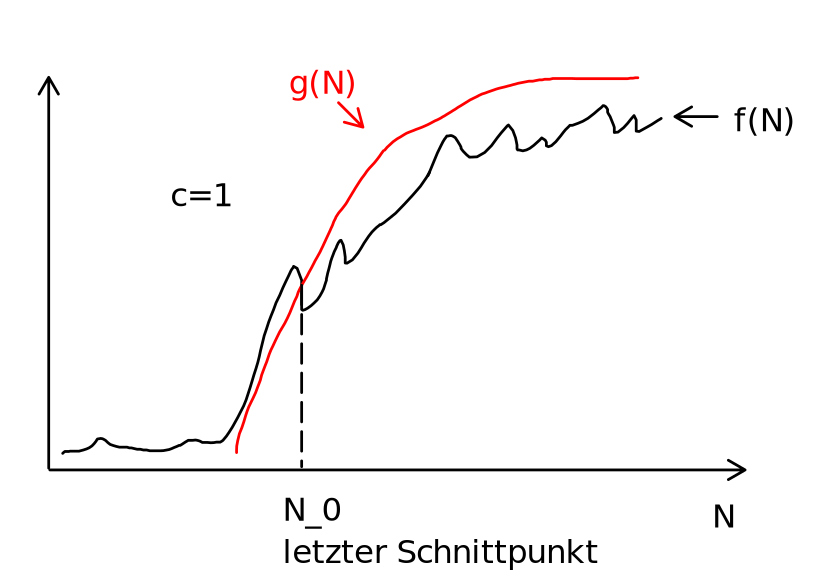
\includegraphics[width=8cm,height=5cm,keepaspectratio]{./Pictures/Komplexitaet.png}

\[\mathcal O(g(N)) := \biggl\lbrace f(N), \text{ so dass } \exists N_0, c \text{ mit } f(N) \leq c * g(N) \text{ für } N \geq N_0 \biggr\rbrace\]

Eigenschaften:
\begin{itemize}
    \item transitiv: $f(N) \in \mathcal O(g(N)) \land g(N) \in \mathcal O(h(N)) \Rightarrow f(N) \in \mathcal O(h(N))$
    \item additiv: $f(N) \in \mathcal O(h(N)) \land g(N) \in \mathcal O(h(N)) \Rightarrow f(N) + g(N) \in \mathcal O(h(N))$
    \item skalare Multiplikation: $f(N) \in \mathcal O(g(N)) \Rightarrow c* f(N) \in \mathcal O(g(N)) $
\end{itemize}

$\Rightarrow$ für Monome und Polynome gilt:
\[ x^k \in \mathcal O(x^{k+j}) \hspace*{2cm} a_0 + a_1x^1 + a_2x^2 + \dots + a_kx^k \in \mathcal O(x^k)\]
für alle $j \geq 0$ \\
Logarithmus: die Basis ist egal, d.h. $log_a(x) \in \mathcal O(log_b(x))$ für alle $a,b >1$
\[ \text{ weil  }\hspace*{1cm} log_a(x) = \frac{log_b(x)}{log_b(a)} \Rightarrow c = \frac{1}{log_b(a)}\]
Aus Multiplikation folgt auch\hspace*{1cm} $c* \mathcal O(f(N)) \in \mathcal O(f(N))$ \\
\hspace*{6cm} $\mathcal O(c*f(N)) \in \mathcal O(f(N))$ \\

mehrere $\mathcal O$'s verschwinden: $ \mathcal O( \mathcal O(f(N)) \in \mathcal O (f(N))$ \\

Spezialfall von Polynom: additive Konstanten dominieren nie \\
\hspace*{1cm}$\Rightarrow$ können weggelassen werden: $\mathcal O(f(N)) + p \in \mathcal O(f(N))$

\section*{5.3 Landau-Symbole, O-Notation}
\addcontentsline{toc}{section}{5.3 Landau-Symbole, O-Notation}
\begin{itemize}[label={}]
    \item groß-$\bigO{}$: \hspace*{5mm}$f(N)$ \glqq $\leq$\grqq $g(N)$ : $\exists N_0, c, $ so dass $\forall N \geq N_0$ gilt : $f(N) \leq c * g(N)$\\
    \hspace*{4.5cm}$\Leftrightarrow f(N) \in O(g(N))$

    \item klein-o:  \hspace*{5mm}$f(N)$ \glqq $<$\grqq $g(N) $: $\underline{\text{ für alle } c>0} : \exists N_0 $, so dass $\forall N \geq N_0$ gilt : $f(N) < c * g(N)$\\
    \hspace*{4.5cm}$\Leftrightarrow f(N) \in o(g(N))$

    \item $\Omega$:  \hspace*{5mm}$f(N)$ \glqq $\geq$\grqq $g(N)$ : $\exists N_0, c, $ so dass $\forall N \geq N_0$ gilt : $c *f(N) \geq  g(N)$\\
    \hspace*{4.5cm}$\Leftrightarrow f(N) \in \Omega (g(N))$

    \item $\omega$:  \hspace*{5mm}$f(N)$ \glqq $>$\grqq $g(N)$ : für alle $\infty > c > 0:$ $\exists N_0, $ so dass $\forall N \geq N_0$ gilt : $c* f(N) > g(N)$\\
    \hspace*{4.5cm}$\Leftrightarrow f(N) \in \omega (g(N))$

    \item $\Theta$:  \hspace*{5mm}$f(N)$ \glqq $=$\grqq $g(N)$ : $\exists N_0, c_1, c_2, $ so dass $\forall N \geq N_0$ gilt : $c_1 * g(N) \leq f(N) \leq c_2 * g(N) $\\
    \hspace*{4.5cm}$\Leftrightarrow f(N) \in \Theta (g(N))$ $\Leftrightarrow f(N) \in \bigO{} (g(N))$ $\land f(N) \in \Omega (g(N))$

    \item $\Rightarrow$ wenn  $f(N) \in o(g(N)) \Rightarrow f(N) \in O(g(N))$ \\
    Beispiele: $N \in o(N^2) \hspace*{0.6cm} \Rightarrow N \in O(N^2)$ \\
    \hspace*{0.65cm} aber: $N \not\in o(N) \hspace*{0.6cm} , \text{aber }N \in O(N)$\\
\end{itemize}

\subsection*{Anwendung auf Sortieren:}
Anzahl der Vergleiche bei :
\begin{itemize}
    \item insertion sort:
    \begin{itemize}
        \item typischer Fall: $V(N)= \frac{N(N-1)}{4} = \frac{N^2}{4} - \frac{N}{4} \in \bigO{}(N^2)$ \\
        \item schlechter Fall: $V(N) = \frac{N(N-1)}{2} = \frac{N^2}{2} - \frac{N}{2} \in  \bigO{}(N^2) $\\
    \end{itemize}
    \item quick sort:
    \begin{itemize}
        \item typischer Fall: $V(N) = 2(N+1) ln(N+1) \in \bigO{}(N*log N)$
        \item schlechter Fall: $V(N) = V(N) = \frac{(N+1)(N+2)}{2} \in \bigO{}(N^2) $\\
    \end{itemize}
\end{itemize}

\subsection*{Rechenregeln}
siehe vorige VL (oder Skript)

\subsection*{Regeln zur Anwendung auf Algorithmen}
\begin{itemize}
    \item Sequenzregel $\widehat{=}$ Nacheinander-Ausführung von Befehlen im Algorithmus \\
    anschauliche Bedeutung: der langsamste Befehl bestimmt die Komplexität \\
    $\begin{rcases}
    \text{Befehl 1} & \bigO{}(f(N)) \\
    \text{Befehl 2} & \bigO{}(g(N))\\ \end{rcases} \bigO{}(f(N)) + \bigO{}(g(N)) \begin{cases}
    \in \bigO{}(f(N)) & \text{ wenn } g(N) \in \bigO{}(f(N)) \\
    \in \bigO{}(g(N)) & \text{ wenn } f(N) \in \bigO{}(g(N)) \\ \end{cases}$ \\
    \hspace*{6.5cm} $\widehat{=} \text{max}(\bigO{}(f(N)), \bigO{}(g(N)))$
    \item Schachtelungsregel $\widehat{=}$ Ausführung eines Befehls (oder einer Sequenz) in einer Schleife \\
    anschauliche Bedeutung: Komplexität erhöht sich um die Anzahl der Durchläufe \\
    $\begin{rcases}
    \text{for k in range(N)}: & \bigO{}(N)\hspace*{3mm} \textcolor{blue}{\bigO{}(f(N))}\\
        \text{  Befehl} & \bigO{}(g(N)) \end{rcases}\bigO{}(N*g(N)) \hspace*{3mm} \textcolor{blue}{\bigO{}(f(N)*g(N))}$
        \item Wie berechnet man die Komplexität?
        \begin{itemize}
            \item vollständige Induktion:
            \begin{enumerate}
                \item Induktionsanfang: suche $N_0$ und $c$, so dass $f(N_0) \leq c*g(N_0)$
                \item Induktionsschritt: falls $f(N) \leq c*g(N)$ \\
                \hspace*{3cm} $\Rightarrow f(N+1) \leq c*g(N+1)$
            \end{enumerate}
            \item Grenzwertbildung $n \rightarrow \infty$ ($\widehat{=}$ alternative Definition von $\bigO{}$, o, etc.)
            \begin{itemize}[label={}]
                \item $f(N) \in \bigO{}(g(N)) \Leftrightarrow \lim\limits_{N \rightarrow \infty} \frac{f(N)}{c*g(N)} = 1$ für ein geeignetes $c \Leftrightarrow \lim\limits_{N \rightarrow \infty} \frac{f(N)}{g(N)} = c$
                \item $f(N) \in o(g(N)) \Leftrightarrow \lim\limits_{N \rightarrow \infty} \frac{f(N)}{g(N)} = 0$
            \end{itemize}
        \end{itemize}
    \end{itemize}

\textbf{Beispiel}: ist log(N) $\in \bigO{}(N)$, Grenzwertmethode:\\
\[\lim\limits_{N\rightarrow\infty} \frac{ln N}{N} = \frac{\infty}{\infty} \text{ ??} \]\\
Regel von l'Hospital: $\lim\limits_{x \rightarrow x_0} \frac{f(x)}{g(x)} = \lim\limits_{x \rightarrow x_0} \frac{f'(x)}{g'(x)}$ falls $\frac{f(x_0)}{g(x_0)}$ unbestimmt

\[f(N) = ln(N) \Rightarrow f'(N) = \frac{1}{N} \hspace*{1cm} g(N) = N \Rightarrow g'(N) = 1 \]
\[\lim_{N \rightarrow \infty} \frac{ln N}{N} = \lim_{N \rightarrow \infty} \frac{\frac{1}{N}}{1} = \lim_{N \rightarrow \infty} \frac{1}{N} =  \frac{''1''}{\infty} = 0  \]
\[ \Rightarrow ln N \in o(N) \]

\section*{5.4 Analyse von Algorithmen für den gleitenden Mittelwert}
\addcontentsline{toc}{section}{5.4 Analyse von Algorithmen für den gleitenden Mittelwert}
\begin{minted}{python}
def running_mean(a, k):             #N=len(a)
    r = [0] * len(a)                #O(N)
    if k > len(a):                  #O(1)
        raise RuntimeError("k too large")
    for j in range (k-1, len(a)):   #O(N-k+1) = O(N)
        for i in range(j-k+1, j+1): #O(k)
            r[j] += a[i]            #O(1) + O(1) + O(1) = O(1)
        r[j] /= float(k)            #O(1) + O(1) + O(1) = O(1)
    return r
\end{minted}
Schachtelung: $\bigO{}(k) * \bigO{}(1) = \bigO{}(k)$ \\
Schachtelung: $\bigO{}(N) * \bigO{}(k) = \bigO{}(N*k)$ \\
Sequenz:      $\bigO{}(N)+\bigO{}(1)+\bigO{}(N*k)+\bigO{}(1) = \bigO{}(N*k)$ \\

Verwende ungünstige Datenstruktur für a: \\
verkettete Liste: a[i] $\rightarrow$ get\_element(a,i) \hspace*{1cm} O(i)\\

\subsection*{Verkettete Liste}
für jedes Element: Node-Datenstruktur, enthält das Datenelement und einen zeiger/Referenz auf den nächsten Node \\

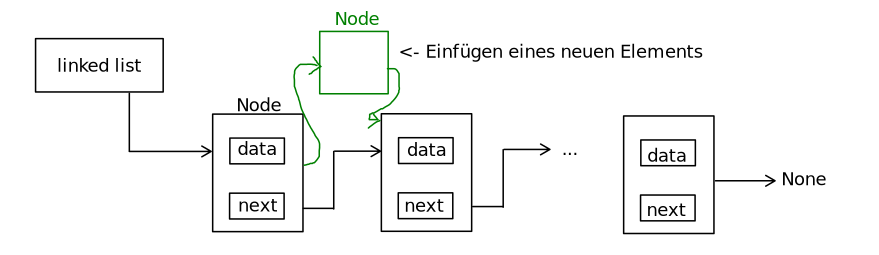
\includegraphics[width=15cm,height=9cm,keepaspectratio]{./Pictures/linkedlist.png}

Zugriff auf Element i: Durchlaufen der Kette bis Node i $\in \bigO{}(i)$ Schritte \\

Zugriff auf Element i: Durchlaufen der Kette bis Node i $\in O(i)$ Schritte \\

\textbf{Optimierte Version des gleitenden Mittels:}
\begin{minted}{python}
def running_mean_2(a, k):             #N=len(a)
    r = [0] * len(a)                  #O(N)
    if k > len(a): ...                #O(1)
    for i in range(k):                #O(k)
        r([k-1] += a[i]               #O(1) -> O(k*1)
    for j in range(k, len(a)):        #O(N)
        r[j] = r[j-1] - a[j-k] + a[j] #O(1) -> O(N)
    for j in range(k-1, len(a)):      #O(N)
        r[j] /= float(k)              #O(1) -> O(N)
    return r                          #Sequenz: maximum-> O(N) (statt O(N*k))
\end{minted}

Rechenregel: $a_0 + a_1 * N + a_2 * N^2 + \cdots + a_k * N^k \in \bigO{}(N^k)$ \\
    \hspace*{3cm} $\bigO{}(N-k) = \bigO{}(N)$


\section*{5.5 Amortisierte Komplexität}
\addcontentsline{toc}{section}{5.5 Amortisierte Komplexität}
\begin{itemize}
    \item falls dieselbe Operation manchmal schnell und manchmal langsam ist:
    \begin{itemize}
        \item wie ist das Verhalten im Mittel?
        \item Verteilt (\glqq amortisiert \grqq) sich der Aufwand von wenigen langsamen Aufrufen über viele schnelle Aufrufe?
    \end{itemize}
\end{itemize}
Anwendung: \textbf{dynamisches Array}
\begin{itemize}
    \item \textbf{Problem}: Einfügung neuer Elemente in ein statisches Array teuer: \\
    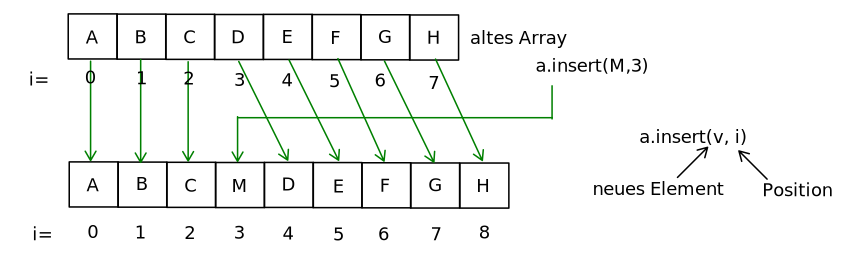
\includegraphics[width=12cm,height=9cm,keepaspectratio]{./Pictures/dynamischesArray.png}
    \begin{enumerate}
        \item neues Array mit einer zusätzlichen Speicherstelle allozieren
        \item die alten Daten kopieren $\Rightarrow \bigO{}(N)$ teuer!
        \item das neue Element einfügen
    \end{enumerate}
    \item \textbf{Lösung}: oft genügt es, wenn neue Elemente immer am Ende angehängt werden
    \item \textbf{Trick}: man alloziert \textbf{mehr} Speicher als man aktuell benötigt (z.B. 2x)
    \item \textbf{Fall 1}: Array hat noch unbenutzten Speicher: \\
    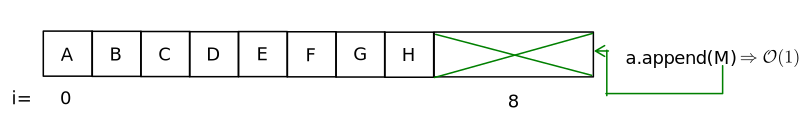
\includegraphics[width=12cm,height=9cm,keepaspectratio]{./Pictures/dynArrunbenutzt.png}
    \item \textbf{Fall 2}: Array ist voll $\Rightarrow$ kopiere in ein neues Array mit \textbf{doppelter} Größe \\
    (nicht: in ein neues Array mit einem zusätzlichen Element, wie in Beispiel 1) \\
    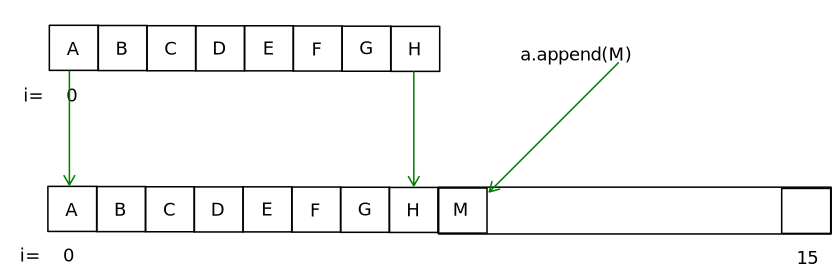
\includegraphics[width=12cm,height=9cm,keepaspectratio]{./Pictures/dynArrDopp.png}
    \begin{enumerate}
        \item alloziere Array der doppelten Größe
        \item kopiere die alten Daten \hspace*{3cm} \textcolor{blue}{$\bigO{}(N)$}
        \item kopiere neues Element  \hspace*{3.1cm} \textcolor{blue}{$\bigO{}(1)$} \\
        $\Rightarrow$ \textcolor{blue}{$\bigO{}(N)$}
    \end{enumerate}
    $\Rightarrow$ jetzt sind noch N-1 Speicherstellen frei (N-1 $\widehat{=}$ alte Arraygröße) \\
    $\Rightarrow$ jetzt bekommen wir (N-1)-mal Fall 1 mot $\bigO{}(1)$
    $\Rightarrow$ selten $\bigO{}(N)$, häufig $\bigO{}(1)$$\Rightarrow$ Was bedeutet das im Durchschnitt?

    \item Was ist die amortisierte Komplexität des \glqq Verdopplungs-Trick\grqq ?
    \item Accounting-Methode: definieren \glqq Guthaben\grqq, das wir während des billigen Anfügens ansparen und bei teuren Operationen verbrauchen \\
    $\varphi_i = \text{size}_i - \text{capacity}_i \leq 0$ weil size $\in$ capacity
\end{itemize}

Kosten einer Einfügung $c_i = \tilde{c_i} + \varphi_i - \varphi_{i-1}$\\
\begin{itemize}
    \item $c_i$ $\rightarrow$ tatsächliche Kosten der Einfügung
    \item $ \varphi_i - \varphi_{i-1}$ $\rightarrow$ verbrauchtes Guthaben
\end{itemize}

\begin{itemize}
    \item \textbf{Fall 1:} vor der i-ten Einfügung gilt size$_{i-1} < \text{capacity}_{i-1} \Rightarrow$ noch Platz
    \begin{itemize}[label={$\Rightarrow$}]
        \item $\tilde{c_i} = 1$ für das Kopieren des neuen Elements, capacity$_i = \text{capacity}_{i-1}$
    \end{itemize}
    $c_i = 1 + (\underbrace{\text{size}_i}_{\text{size}_{i-1}+1}- \text{capacity}_i) - (\text{size}_{i-1} - \text{capacity}_{i-1}) = 2$

    \item \textbf{Fall 2:} vor der i-ten Einfügung gilt: $\text{size}_{i-1} = \text{capacity}_{i-1} \Rightarrow $ Array voll \\
    \hspace*{7.8cm}  $\text{capacity}_{i} = 2*\text{capacity}_{i-1} $ \\
    \begin{itemize}[label={$\Rightarrow$}]
        \item   $\tilde{c_i} = \hspace*{-2.3cm}\underbrace{\text{size}_{i-1}}_{\text{alte Elemente in den neuen Speicher kopieren}}\hspace*{-2.3cm}+  1 \leftarrow$ neues Element kopieren
    \end{itemize}
    $c_i = \text{size}_{i-1} + 1 + (\underbrace{\text{size}_{i}}_{\text{size}_{i-1}+1} - \hspace*{-0.3cm} \underbrace{\text{capacity}_{i}}_{2*\text{capacity}_{i-1} = 2* \text{size}_{i-1}}\hspace*{-0.5cm}) - (\text{size}_{i-1} -\underbrace{ \text{capacity}_{i-1}}_{\text{size}_{i-1}}) = 2$ \\

    in beiden Fällen: $c_i = 2 \Rightarrow$ amortisierte Komplexität $\bigO{}(1)$
\end{itemize}

\begin{tabular}{l | C{0.5cm} C{1.5cm} | C{2cm} | C{1.5cm} | C{2.6cm}| C{1cm} | C{1.5cm}}
    Array & size & capacity & aktuelle Kosten $\tilde{c_i}$ & totale Kosten &  Durchschnitts- kosten & $\varphi_i$  & $c_i = \tilde{c_i} + \varphi_i - \varphi_{i-1}$\\\hline
    \mintinline{python}{[None]} & 0 & 1 & & & & -1 & \\
    \mintinline{python}{[a]} & 1 & 1 & 1 & 1 & 1 & 0 & 2\\
    \mintinline{python}{[a,b]} & 2 & 2 & 1+1 & 3 & 3/2 & 0 & 2\\
    \mintinline{python}{[a,b,c, None]} & 3 & 4 & 2+1 & 6 & 6/3 & -1 & 2\\
    \mintinline{python}{[a,b,c,d]} & 4 & 4 & 0+1 & 7 & 7/4 & 0 & 2\\
    \mintinline{python}{[a,b,c,d,e,None,None,None]} & 5 & 8 & 4+1 & 12 & 12/5 & -3 & 2 \\
    \mintinline{python}{[a,b,c,d,e,f,None,None]} & & & & &&-2 & 2\\
    \mintinline{python}{[a,b,c,d,e,f,g,None]} & & & & && -1 & 2\\

\end{tabular}


